\chapter{Krav}

På baggrund af et møde med Jim Jensen fra Hammel Neurocenter, som er projektets udbyder, hvor udfordringer med nuværende behandlinger og udredninger af dysfagipatienter blev diskuteret, er der udarbejdet en kravspecifikation til et system kaldet Synkerefleksmonitor (SRM). Formålet med mødet var ikke at etablere kunde/leverandør- relation, hvor krav til et kommende produkt skal forhandles på plads. Mødet havde i stedet en uformel karakter, hvor Hammel Neurocenter frivilligt er gået med til at mødes med gruppens medlemmer for at bidrage med deres ekspertise indenfor behandling og udredning af dysfagipatienter. Kravene til produktet som skal realiseres under dette projekt, er suverænt udspecificeret af gruppens medlemmer uden indblanding af projektets udbyder. Fra udbydernes side var der kun et ønske om at bidrage med udvikling af nye metoder til udredning af dysfagipatienter, hvilken dette projekt også har intentioner om. \\

I det følgende beskrives kort det overordnede system, efterfulgt af funktionelle og ikke funktionelle krav.  

\section{Systembeskrivelse}
Systemet består af et BI kredsløb og en kommerciel EMG-måler, der tilsammen udgør SRM'en, se figur \ref{fig:sysbeskrivelse}. SRM'en initieres af et sundhedspersonale ved første at tilkoble elektroder fra hhv. BI- og EMG-måleren til et raske måleobjekt. Derefter igangsætter sundhedspersonalet målingerne via. en brugergrænseflade på en PC. Begge målinger kører simultant. Efterfølgende opsamles målingerne i et A/D-konverter, der omsætter de målte værdier fra analoge til digitale værdier, som PC'en kan arbejde med. I PC'en processeres de to målinger og vises til sundhedspersonalet via. brugergrænsefladen.   

\begin{figure}[H]
\centering
{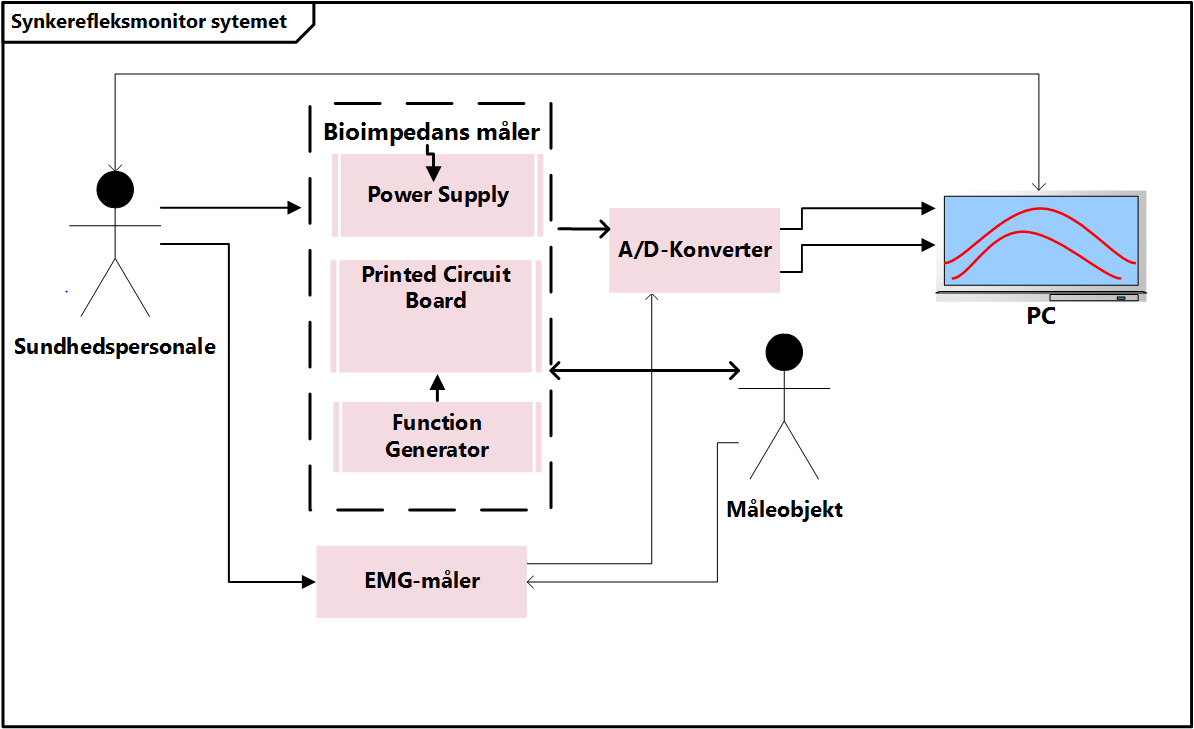
\includegraphics[width=10cm]
{Figure/AktoerKontextDiagram}}
\caption{Aktør-kontekst diagram illustrer det overordnet systemet, som betsår af to måleapparater, en A/D-konverter og en PC. Et sundhedspersonale igangsætter målingerne via. en brugergrænseflade. Måleobjektet er tilkoblet til begge apparater. }
\label{fig:sysbeskrivelse}
\end{figure}  

 

\section{Aktørbeskrivelse}
Til aktør-kontekst diagrammet følger der en en aktør beskrivelse, der beskriver kort hver komponentes funktion, se tabel \ref{tab:aktoerbeskrivelse}.    

\begin{table}[H]
\begin{tabularx}{\textwidth}{l l X}
     Aktørnavn	&	Type		&	Beskrivelse \\ \midrule
     Sundhedspersonale   	&  	Primær  	& 	Sundhedspersonalet tilkobler BI- og EMG-måleren til måleobjektet vha. elektroder, samt starter målingen. Yderligere interagerer sundhedspersonalet med en brugergrænseflade.     \\ 			  \addlinespace[2mm]
     Bioimpedans-måler	&	Sekundær	& BI- måleren anvendes til at måle bioimpedans signaler fra måleobjektet  	 \\   \addlinespace[2mm]

  EMG-måler	&	Sekundær	&	EMG-måleren anvendes til at måle EMG signaler fra måleobjektet.
     \\   \addlinespace[2mm]
    
    Måleobjekt	&	Sekundær	&	Måleobjektet er kilden  hvorfra biosignalerne indhentes. Måleobjektet er tilkoblet til både BI- og EMG-måleren.
     \\   \addlinespace[2mm]
     
 A/D-konverter	&	Sekundær	&	A/D-konverterens funktion er at konvertere analoge signaler fra hhv. BI-og EMG-måleren  til digitale signaler.
     \\   \addlinespace[2mm]      
    PC	&	Sekundær	&	Denne brugergrænseflade bruges til at visualisere de målte signaler i graf form.
     \\   \addlinespace[2mm]
     
   
     \bottomrule                                                                                                                   
    \end{tabularx}
    \caption {Aktørbeskrivelse for det samlede system}
    \label{tab:aktoerbeskrivelse}
	
\end{table}


\section{Funktionelle krav}

Nedenstående tabel 2.2 beskriver funktionelle krav, der stilles til applikationen synkerefleksmonitor. Nogle krav er vigtigere end andre, og de prioriteres vha. MosCow-metoden. Kravene i Must og Should prioriteres højest. I dette projekt bestræbes det at opfylde kravene i Must og Should


\begin{table}[H]

\begin{tabularx}{\textwidth}{X|X}
\rowcolor{Gray}
\toprule
\textbf{Must have} & \textbf{Should have} \\
\hline \\
\textbf{1. }Systemet skal have en bioimpedans sensor (BI), der kan måle bioimpedans signaler & \textbf{5. }Validere bioimpedans sensoren op imod kommerciel BI måler \\[5ex]
\textbf{2. }Systemet skal have EMG sensor, der kan måle EMG signaler & \textbf{6. }Matlab GUI, der kan præsentere BI og EMG signaler \\[3ex]
\textbf{3. }Systemet skal kunne vise BI og EMG signaler over tid på en graf (offline) i Matlab  & \textbf{7. }Både BI og EMG målinger skal køre simultant\\[4ex]
\textbf{4. }Systemet skal kunne beregne BI på baggrund af målte spændinger & \\[4ex]


\midrule
    \rowcolor{Gray}
    \textbf{Could have} & \textbf{Would have}\\
    \midrule \\
\textbf{8. }Real-time visning af EMG- og BI signalerne & \textbf{10. }Mobilt synkerefleksmonitor med touch skærm\\[4ex]
\textbf{9. }Machine Learning for at diskriminere mellem synkerefleks og støj (tale og hoste)& \textbf{11. }EMG og BI signalerne overføres til EPJ  \\[4ex]
& \textbf{12. }Tage højde for anatomiske forskelle mellem kønnene\\[4ex]

\end{tabularx}

\caption{MoSCoW analyse af synkerefleksmonitor}
  \label{tab:moscow}
\end{table}




